\chapter[HEALTH AND ENVIRONMENT]{\textbf{HEALTH AND ENVIRONMENT}}
\thispagestyle{empty}
\numberwithin{equation}{chapter}



\section{DYNAMICS OF TUMOUR GROWTH}

\par ~~~~~~~~~~~~Tumor growth is a complex process ultimately dependent on tumor cells proliferating and spreading in host tissues. The current view of tumor growth kinetics is based on the general assumption that tumor cells grow exponentially (Shackney, 1993). Lower than expected activity of tumor cells and greater than expected aneuploidy have also been consistently found. These issues are of great importance since both radiotherapy and chemotherapy are entirely based on cytokinetics.

\par ~~~~~~~~Mathematical modelling of tumor growth expresses the dependence of tumor site on time. Given the population of the tumor, let x be the number of individual cells at time t. It has been observed experimentally that free-living dividing cells, such as bacteria cells, grow at a rate proportional to the volume of dividing cells at that moment.
\newline Hence   we  have  a  differential equation, $ \frac{dx}{dt}=\lambda x $ 


\par ~~~~~~~~~~~~The population x is positive and increasing due to different biological factors and mutation and so
 $ \frac{dx}{dt}>0 $    
and $\lambda >0$ with the following initial condition $ x(t_{0})=xo $.
          
~~~~~~Now by variable separable method and the solution is $ x=x_{0}e^{y(t-to)} $.
%
Thus, free-living dividing cells grow exponentially with time, and this law of population tumor growth is called \textit{Malthusian Law}. This equation  is  a  good  model  of tumor for the earliest stage of growth. Here $y$ is related to the tumor’s doubling time. That is the volume of cells keeps doubling every time interval of length $ \ln\frac{2}{\lambda}$

\subsection{Gompertzian relation}


\par ~~~~~~~~Solid tumours do not grow exponentially with time. As the tumour becomes larger, the doubling time of the total tumour volume continuously increases. A number of researchers have shown that the data for many solid tumours is fitted remarkably well, over almost a thousand-fold increase in tumour volume, by the equation                  
$$ x(t)=x_{0} e^{\frac{\lambda}{a} (1-e^{-at})} $$                                  
where $ \lambda $ and a are positive constants. The above equation is usually known as a Gompertzian relation. It states that tumour grows more and more slowly with the passage of time, and that it ultimately approaches the limiting volume $ x_{0}e^{\frac{\lambda}{a}} $. 

\par ~~~~~~~~~~~~Medical scientists have long been concerned with explaining this deviation from simple exponential growth. An insight into this  problem can be gained by finding a differential equation satisfied by $ x(t) $.    
%
%
\\
ie, $$\frac{dx}{dt}=x_{0} \lambda e^{(-at)} e^{\frac{\lambda}{a} (1-e^{-at})} $$
$$ =\lambda e^{(-at)}x $$
               
 \par ~~~~~~Two theories have been evolved for the  dynamics of tumour growth. They corresponds to the two  arrangements of above equation as
 $$ \frac{dx}{dt}=(\lambda e^{(-at)})x  $$
 $$ \frac{dx}{dt}=\lambda (e^{(-at)}x) $$







According to the first theory, the retarding effect of tumour growth is due to an increase in the mean generation time of the cells,   without a change in the proportion of reproducing cells. As time goes on, the   reproducing cells mature or age, and thus divide more slowly.

\par   ~~~~~~~~On the other hand, the second theory corresponding to the second equation, suggests that the mean generation time of the dividing cells remains constant, and the retardation of growth is due to a loss in reproductive cells in the tumour. One possible explanation for this is that a necrotic region develops in the centre of the tumour. This necrosis appears at a critical size for a particular type of tumour, and thereafter the necrotic "core" increases rapidly as the total tumour mass increases. According to this theory a necrotic core develops because in many tumours the supply of blood, and thus of oxygen and nutrients, is almost completely confined to the surface of the tumour and a short distance beneath it. As the tumour grows, the supply of oxygen to the central core by diffusion becomes more and more difficult resulting in the formation of a necrotic core.

\subsection{Kuznetsov et al model}

\par ~~~~~~~~~~~~~~The tumor cell population growth is represented more realistically in many cases by assuming that the number $x(t)$ of individual cell in the population at time t is described by a Bernoulli Equation of the form $ \frac{dx}{dt}=\alpha t-\beta t^{2} $ where $ \alpha >0$ and $ \beta >0 $ are constants.    
$- \beta x^{2} $ is added due to the cause that tends to minimize the ultimate growth of the population. Such a cause could be the radiation therapy, chemotherapy or biological therapy when the population becomes sufficiently large as the tumor grows which has a quadratic affect on the individual cell. 

\par ~~~~~~~~~~~~Let us assume that the tumor cell population is described by a differential equation $ \frac{dx}{dt}=\alpha t-\beta t^{2} $  with constants  $ \alpha >0$ and $ \beta >0 $ and initial condition $ x(t_{0})=x_{0} $ .
 In some cases, $\beta $ is very small compared to $\alpha $. Hence, for a sufficiently small number x, the term $\alpha x $ predominates and so the tumor cell population grows very rapidly for that time period. However, as the tumor grows by diffusion and x becomes sufficiently large, the term $ \beta x^{2} $ is of greater influence and the result of this is a decrease in the rapid growth rate.
 
The law of population growth so described is called the logistic law of cancer tumor growth. 
 $ ~~~~~~~~\frac{dx}{dt}=\alpha x-\beta x^{2} $ $~~~~~~~~~~\Rightarrow $ 
$~~~~~~~~~~ \dfrac{dx}{\alpha x-\beta x^{2}}=dt $ 

Using partial fraction and applying the initial conditions, we get
$$ x=\dfrac{\alpha y_{0} e^{y(t-t_{0})}}{1+\beta y_{0} e^{y(t-t_{0})}} $$ 
where $ y_{0}= \dfrac{x_{0}}{\alpha -\beta x_{0}} $ .

\par ~~~~~~~~~~~~Now to see how large the cancer cell population will ultimately be, let us assume $ t\rightarrow \alpha $ and $ x\rightarrow \frac{\alpha}{\beta} $
%
%  
  
\par ~~~~~~~~~~~~The tumor–immune interaction can be modelled using various mathematical methods such as ordinary or partial differential equations. In this context, Kuznetsov et al.  define an ordinary differential equation model for two main populations: effector cells and tumor cells. They predict a threshold above which there is uncontrollable tumor growth and below which the disease is attenuated with periodic exacerbations occurring every 3-4 months. The finlt result gives ordinary differential equation for the populations of immune and tumor cells and they show that survival increases if the immune system is stimulated.  

 
\pagebreak

\section{DETECTION OF DIABETES}

\par ~~~~~~~~~~The human body needs to maintain a level of glucose concentration that is not too high in order for it to function properly. In order for glucose to be produced and utilized, insulin production and utilization must occur. If insulin is not produced, or not enough of it is produced then proper glucose levels cannot be maintained, which leads to the disease of diabetes. Diabetes mellitus is a condition in which there is too much glucose in our blood.

\par ~~~~~~~~~~In diabetes, the body is unable to burn off all its sugar,starches and carbohydrates due to insufficient supply of insulin. Diabetes is usually diagnosed by fasting and post periodical blood test or by glucose tolerance test(GTT). In GTT, the patient after fasting overnight is given a large dose of glucose,and during the next three to five hours several measurements are made of the concentration of glucose in the, patient's blood.

\par  ~~~~~~~~~~In the mid-sixties, Dr.Rosevear and Dr.Molnar, Dr.Ackerman and Dr.Gatewood discovered a criterion for interpreting the results of GTT. Their model is based on the following simple and well known facts of elementary biology.

\begin{itemize}
	
	\item  Glucose is a source of energy for all tissues and organs. For each individual there is an optimal blood glucose concentration. Any excessive deviations from this optimal concentration leads to severe pathological conditions and potential death.
	\item  Blood glucose levels are influenced and controlled by a various of hormones and metabolism such as the following: 
	
	(i) \textit{insulin}, a hormone secreted by $ \beta $ cells of the pancreas. After absorbing carbohydrates, the pancreas secretes more insulin. In addition, the glucose in the blood directly stimulates the $ \beta $ cells to secrete insulin. Insulin facilitates the tissue uptake of glucose. Without sufficient insulin, the body cannot have all the energy it needs.\\
	
	(ii) \textit{Glucagon}. It is a hormone secreted by the $ \alpha $ cell of the pancreas. Any excess glucose is stored in the liver in the form of glycogen and when needed this glycogen in converted back into glucose. The hormone glucagon increases the rate of breakdown of glycogen into glucose. Evidences have shown that hypoglycaemia(low blood sugar) and fasting promote the secretion of glucagon while increased blood glucose levels suppresses its secretion.\\
	
	(iii) \textit{Epinephrine (adrenalin)}. This is a hormone secreted by the adrenal medulla, and is a part of the emergency mechanism to quickly increase the concentration of glucose in the blood in case of extreme hypoglycaemia. It also increases the rate of breakdown of glycogen into glucose like glucagon, but in addition, it directly inhibits glucose uptake by muscle tissues it-acts directly on the pancreas to inhibit insulin secretion. It also aids in the conversion of lactate to glucose in the liver.\\
	
	(iv) \textit{Glucocorticoids} are hormones, such as cortisol, which are secreted by the adrenal cortex. These hormones play an important role in the metabolism of carbohydrates.\\
	
	(v) \textit{Thyroxin} is a hormone secreted by the thyroid gland. It helps the liver .to form glucose from non carbohydrate sources such as glycerol, lactate and amino acids.\\
	
	(vi) \textit{Growth hormone (somatotropin)}. This is a hormone secreted by the anterior pituitary gland. This hormone not only affects glucose level in a direct manner, but also tends to block insulin. These hormones decrease the sensitivity of muscle and adipose membrane to insulin,thereby reducing the effectiveness of insulin in promoting glucose uptake.	
\end{itemize}

\subsection*{Mathematical model}
\par ~~~~~~~~~~The model Postulated is a simple one, requiring only a limited number of blood sample during a GTT, and it centres on two concentrations: \\
(a) G (glucose in the blood), and \\
(b) H (net hormonal concentration). \\
\linebreak
The latter represents the commutative effect of all the important hormones. Insulin  is considered to increase H while cortisone decreases H. Then the basic model is described by the equations     

~~~~$$~~~~~~\frac{dG}{dt}=F_{1}(G,H)+J(t)$$
$$\frac{dH}{dt}=F_{2}(G,H)~~~~$$ 
where J(t) is the external rate at which the blood glucose concentration is being increased.
\par ~~~~~~~~~~~~We assume that by the time a fasting patient arrives in the hospital, G and H have achieved the equilibrium values $G_{0}$ and $H_{0}$ (say).
\\ ie,           $F_{1}(G_{0},H_{0})=0=F_{2}(G_{0},H_{0})$  .
We are now interested in deviations of G and H from their equilibrium values, so we take $G=G_{0}+g$ and $H=H_{0}+h$ where g and h are small as compared to $G_{0}$ and $H_{0}$.\\ Then,

$~~~~~~~~~~~~\frac{dg}{dt}=F_{1}(G_{0}+g,H_{0}+h)+J(t) 
=f_{1}(g,h)+J(t)$      ~~~~~~~~~~~~~~~~~~            (say) \\

$~~~~~~~~~~~~~~~~~~\frac{dh}{dt}=f_{2}(g,h)$~~~~~~~~~~   (say) \\

We also assume that $f_{1}$, and $f_{2}$ have a linear form.
Thus,
%\begin{equation}
$$\dfrac{dg}{dt}=-ag-bh-J(t)$$
$$\frac{dh}{dt}=-ch+eg$$
%\end{equation}

\par ~~~~~~~~~~Now, $a>0$, since $\frac{dg}{dt}<0$ for h=0 through tissue uptake of glucose, and $b>0$, since $h>0$ tends to decrease blood glucose levels. Also, $c>0$ since the concentration of hormones in the blood decreases through hormone metabolism and $e>0$ for $g>0$ causes the endocrine glands to secrete those hormones that tend $t_{0}$ increase h.


$$h=\frac{1}{b}[-ag+J-\frac{dg}{dt}]$$
$$\frac{d^{2}g}{dt^{2}}+(a+c)\frac{dg}{dt}+(ac+be)g=\frac{dJ}{dt}+cJ$$

The right-hand side of the equation, is zero except over a small interval of time. Let time t=0 be the time glucose load has been ingested so that for $t>0$

$$\frac{d^{2}g}{dt^{2}}+(a+c)\frac{dg}{dt}+(ac+be)g=0$$         

\par  ~~~~~~~~~~The solutions of this  equation are of three different types, depending upon whether $A^{2}-B^{2}$ is positive, negative or zero. These three types correspond to the over damped, critically damped and under damped case discussed earlier. We shall       take here the case $A^{2}-B^{2}<0$ (the other cases may be dealt in a similar manner) and the solution is
$$g=e^{-At}[Ccos(B_{0}t)+Dsin(B_{0}T)]$$ where $B_{0}=B-A$. Thus the complete solution is
$$G=G_{0}+e^{-At}[Ccos(B_{0}t)+Dsin(B_{0}t)]$$          

This contains five constants. Finding them is as follows:\\

~~~~~~~~~~~~~The patient's blood glucose concentration before the glucose load is ingested is $G_{0}$.Hence, we can determine             $G_{0}$ by measuring the patient's blood glucose concentration immediately upon his arrival at the hospital. Next, we take four additional measurements $G_{1}, G_{2}, G_{3} and G_{4}$ at time $t_{1}, t_{2}, t_{3} and t_{4}$. We can then determine A, $B_{0}$, C and D from the four equations given by

$$G_{i}=G_{0}+e^{-At_{i}}[Ccos(B_{0}t_{i})+Dsin(B_{0}t_{i})]~~~~~~~~~~~~~~~~~~~~~~~~i=1,2,3,4$$      

\par ~~~~~~~~~~The second and better way is to take, say n measurements, and use the least squares techniques to find the best fit for the parameters. However, this has to be solved on a computer.

\par ~~~~~~~~~~~~Observation has shown that slight errors in measuring G can produce large errors in the value of A. However, the value of the parameter $B_{0}$ was relatively insensitive to experimental errors in G. So we determine $B_{0}$ and use this value as a basic description for the response to a GTT.  The remarkable fact is that a value for $t_{0}=\frac{2\pi}{B_{0}}$ of less than 4 hours Indicated normality, while appreciably more than 4 hours indicated mild diabetes.




\pagebreak

\section{A PROBLEM IN EPIDEMIOLOGY}




\par ~~~~~~~~~~~~~~~~An important problem in biology and medicine deals with the occurrence, spreading and control of a contagious disease. i.e, one which can be transmitted from one individual to another. The science that deals with this study is called epidemiology, and if a large number of population gets the disease, we say that there is an epidemic. The goal of epidemiologists is first to understand the causes of a disease, then to predict its course, and finally to develop ways of controlling it, including comparisons of different possible approaches.

\subsection*{HISTORY}

\par ~~~~~~~~~~~~The study of infectious disease data began with the work of John Graunt in his 1662 book “Natural and Political Observations made upon the Bills of Mortality”. He analysed the various causes of death and gave a method of estimating the comparative risks of dying from various diseases. What is usually described as the first model in mathematical epidemiology is the work of Daniel Bernoulli on inoculation against smallpox. In the eighteenth century smallpox was endemic. After that another valuable contributions are arrived on the basis of cholera, typhoid etc. In 1840, William Farr studied statistical returns with the goal of discovering the laws that underlie the rise and fall of epidemics. Communicable diseases have always been an important part of human history. 

\par ~~~~~~~~~~~~~~Problems involving the spread of disease can be very complicated. For example, it is known that some individuals may not actually get a disease even when exposed for long periods of time to others having the disease. In such case, we say that the individual has an immunity to the disease either because having had   the disease before he has build up resistance to recurrence or by having initial   resistance (natural immunity) he is not able to contract the disease. In some cases, individuals are immune to a disease but are capable of transmitting it to others; such individuals are called carriers. An example to this effect is the case of typhoid fever.      



\subsection*{MATHEMATICAL MODEL}

\par ~~~~~~~~~~~~~~To have a simple mathematical description for the spread of a disease suppose that there is a large but finite population. Let us restrict ourselves to the students in some large college or university, who remain on campus for a relatively long period and do not have access to other communities. We presuppose that there are     only two types of students, those who have a contagious disease (called infected), and those who do not have the disease, (i.e. unaffected) but are capable of contracting it on exposure to an infected student. If there are some infected students initially, then we want to find a formula for the number of infected students at any time.

\par ~~~~~~~~~~Let $N_{i}$ denote the number of infected students at any time t and $N_{u}$ the uninfected students. Then,if N is the total number of students (assumed to be constant), we have $N=N_{i}+N_{u}$

\par ~~~~~~~~~~~~Here, $\dfrac{dN_{i}}{dt}$ is the time rate of change in the number of infected students and should depend in some way on $N_{i}$, and thus $N_{u}$. Assuming that $\frac{dN_{i}}{dt}$ is a quadratic function of $N_{i}$ as an approximation, we get     
$$\frac{dN_{i}}{dt}=a_{0}+a_{1}N_{i}+a_{2}N_{i}^{2}$$,
where $a_{0}$, $a_{1}$, $a_{2}$ are constants.  \\                                              
\par ~~~~~~~~~~~~Now we would expect, $\dfrac{dN_{i}}{dt}=0$  where $N_{i}=0$, (i.e, there are no infected students) and where $N_{i}=N$, (i.e, all students are infected).      
 \begin{center}
	\begin{eqnarray*}
			Then ~~~~~~~~~~~~~~~~~~~~~~~~~~~~~~~~~~~~~~~~a_{o}&=0 \\
			a_{1}N+a_{2}N^{2}&=0 \\
			a_{2}&=-\frac{a_{1}}{N} 
	\end{eqnarray*}
\end{center}

\begin{center}
	\begin{eqnarray*}
			Hence~~~~~~~~~~~~~~~~~~~~~~~~~~~~~~~~~~~~~~~~~~~~~ \frac{dN_{i}}{dt}&=a_{1}N_{i}-\frac{a_{1}N_{i}^{2}}{N}  \\
			&=\frac{a_{1}}{N}N_{i}(N-N_{i}) \\
	 		&=kN_{i}(N-N_{i})
	 \end{eqnarray*}
\end{center}                   
where $k = \frac{a_{1}}{N}$ and the initial conditions are $N_{i}(t=0)=N_{0}$

$\therefore $
$~~~~~~~~N_{i}=\dfrac{N}{1+[\frac{N}{N_{0}}-1]e^{-kNt}}$
\\
	
\par ~~~~~~~~~~The graph of this solution is the logistic curve. From the shape of the logistic curve we see that initially there is a gradual increase in the number of infected students, followed by a rather sharp rise in their number near the inflection point, and finally a tapering off. The limiting case occurs where all students become infected,  ($N_{i}\rightarrow N$ as $t \rightarrow \infty$). But from a realistic point of view, this would not happen because  the infected students once they are discovered would be isolated so  as to prevent others from contacting it.

\subsection*{EXAMPLE}

	
	
\par ~~~~~~~~~~A student carrying a flu virus returns to an isolated college hostel of 1000 students. If it is assumed that the rate at which the virus spreads is proportional ot only to the number Ni of infected students but also to the students not infected. Find the number of infected students after 6 days when it is further observed that after 4 days $N_{i}(4)=50$.  \\ 


\textit {\Large Solution} \\ 
\par ~~~~~~Assuming that no one leaves the hostel throughout the duration of   the disease, we must then solve the initial value problem
\begin{center}
	\begin{eqnarray*}
		\dfrac{dN_{i}}{dt}&=kN_{i}(N-N_{i}) \\  
	  \	N(0)=1&=kN_{i}(1000-N_{i}) \\
		N_{i}=N(t)&=\frac{1000}{1+999e^{-1000kt}} 
	\end{eqnarray*}
\end{center}

\begin{center}
	Now using~~~~~~~~~~~~~~~~~~~~~~~~~~~~~~~~~~~~~~~~~~~~~~~~~~~~~~~~~~~~~~~~~~~~~~~~~~ 
	\begin{eqnarray*}
			N_{i}(4)&=50 \\
			50&=\frac{1000}{1+999e^{-1000kt}}  \\
	 		e^{-4000k}&=\frac{19}{999}  \\
			k&=0.0009906  
	\end{eqnarray*}
\end{center}

\begin{center}
	$\therefore$ $~~~~~~~~~~~~N_{i}=N(t)=\frac{1000}{1+999e^{-0.9906t}}$
\end{center} 

\begin{center}
		or $N_{i}=N(6)~~~~~~$ 
		$$~~~~~~~~~~~~~~~~=\dfrac{1000}{1+999e^{-5.9436}}$$ 
		$$~~~~~~~~~~=276 students$$  
\end{center}

\newpage
\vspace*{2cm}
Additional calculated values of N(t) are given in the table \\


\begin{center}
\begin{tabular}{|c|c|}
		\hline
		t & N \\
		(Days)&(Number of infected students) \\
		\hline
		4&50(observed) \\
		\hline
		5&124 \\
		\hline
		6&276 \\
		\hline
		7& 507 \\
		\hline
		8&735 \\
		\hline
		9&882 \\
		\hline
		10&953 \\
		\hline
	\end{tabular}
\end{center}
\vspace*{1cm}
Hence logistic curve for infected students is

%GRAPH
\begin{center}
	\scalebox{1.20} % Scale down to 70 /% of the original size!
	{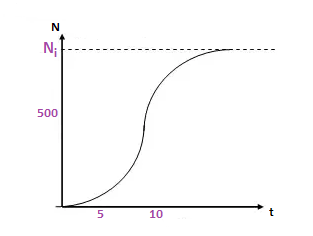
\includegraphics{graph6.png}} 
\end{center}


\pagebreak

\section{CARDIOVASCULAR SYSTEM RESPONSE DYNAMICS TO EXERCISE STRESS}



\par ~~~~~~~~~~One of today’s applied problems which appear in medicine is to predict the heart rate and blood pressure dynamics under exercise stress. This is the main task in the planning process of rehabilitation after the cardiovascular system diseases. This chapter presents a mathematical model of the heart rate and pressure under the influence of physical activity. The work is dedicated to building a model of the pulse and pressure dynamics under the influence of physical activity and the method of their identification.
\subsection*{History}
\par ~~~~~~~~~~~~On the basis of similarities between the cardiovascular system of man and electrical systems O. Frank in the early 20th century suggested modelling the cardiovascular system through an electrical circuit. But,since this approach are the relatively low accuracy and complexity of construction, of identification representation of the cardiovascular system with a system of differential equations acts as much more powerful tool for modelling.

\par ~~~~~~~~~~Well-known paper is based on the use of differential equations that model the work of a four-chambered heart described by Grodins. Also this models takes into account Starling’s and Bowditch’s effects
and self-regulation in the peripheral areas. areas. This model can be used to analyse the blood pressure in a brain and measure blood pressure during orthostatic stress.

\subsection*{Mathematical Model}
\par ~~~~~~~~~~~~Clinical experience has identified two main stages of functioning of the cardiovascular system under exercise stress: period of response of the cardiovascular system to stress and recovery period. The last one is accompanied with increased values of pulse and pressure and they increase in proportion to the intensity of physical activity, while the recovery period makes them return to their original state.


%figure


\begin{center} %Align the Image
	\scalebox{1.00} % Scale down to 70 /% of the original size!
	{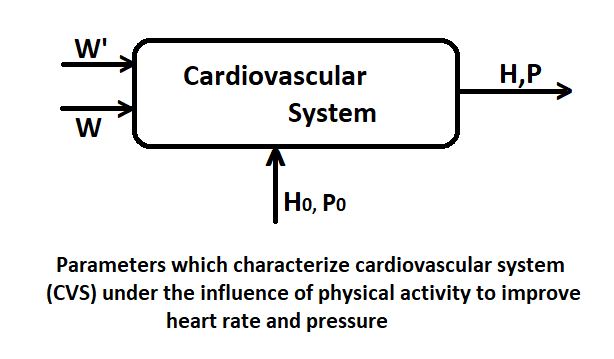
\includegraphics{graph11.png}} %include the image - image is in the working folder
	%\caption{} \label{altbin1} %Caption of the image and label
\end{center}



\par ~~~~~~~~~~~~~The general structure of the model is visualized above. W is load, W' is change of load, H, P are heart rate and blood pressure, $H_{0}, P_{0}$ are initial values of heart rate and blood pressure.
\par The stage of the body’s response to exercise can be selected using the \textit{Michaelis-Menten function}:
$$ M(t)=\frac{M(t)}{1+M(t)}$$
which is a smooth analogue of the Heaviside function. Its value is close to 1 at high volume load and reduced to 0 with a sharp decrease in physical activity. The last activates the body’s recovery process defined as characteristic equal to 1-M(t). The period of the phase transition of the organism from stress to recovery is characterized by certain inertia. It is shown as the delay argument $t-t_{0}$ in the characteristics of the recovery process
$$R(t)=1-M(t-t_{0})$$
$$~~~~~~~~~~~~=1-\frac{W(t-t_{0})}{1+W(t-t_{0})}$$
where $t_{0}$ is transition duration from the time of unloading until the activation process of recovery. 
\par ~~~~~~~~As the pressure changes are proportional to the change of physical activity as $p,h\approx W' $, and their dynamics can be described by the following Cauchy problem for a set of differential equations:
$$h'(t)=A_{1}W'(t) \frac{W(t)}{1+W(t-t_{0})}-(1-\frac{W(t-t_{0})}{1+W(t-t_{0})})A_{2}h^{A_{3}}(t)$$

$$p'(t)=B_{1}W'(t) \frac{W(t)}{1+W(t-t_{0})}-(1-\frac{W(t-t_{0})}{1+W(t-t_{0})})B_{2}h^{B_{3}}(t)$$
\begin{center}
	h(0)=0 \\
	p(0)=0\\	
\end{center}
where $A_{1}$, $B_{1}$ are the indicators of the dynamics of the exercise stress on the change of heart rate and blood pressure; $A_{2}$, $B_{2}$ are the indicators of speed adaptation to exercise stress relieving; $A_{3}$, $B_{3}$ are the coefficients of the heart rate and blood pressure influence in the process of adaptation to unloading; h, p are excess levels of functional heart rate Hm and blood pressure $P_{m}$.
$$h=H-H_{m}$$
$$p=P-P_{m}$$

\subsection*{Identification of Mathematical Model}
\par ~~~~~~~~~~~~The offered mathematical model requires parameter identification, which can be carried out by the root-mean-square criterion. 

$$\vec{a}=\arg \min_{\vec{A}}\sum_{j=1}^{N_{t}}[\tilde{h}(\vec{A},t_{j})-(H_{j}-H_{m})]^{2}$$

$$\vec{b}=\arg \min_{\vec{B}}\sum_{j=1}^{N_{t}}[\tilde{p}(\vec{B},t_{j
})-(P_{j}-P_{m})]^{2}$$

where $N_{t}$ is dimension of the set of points measured for the experiment. $\vec{a}$ ,$\vec{b}$ is the solution of differential equations for a given set of coefficients $\vec{A}$, $\vec{B}$ at the observation
point t.
\par ~~~~~~To minimize the functional let’s use modified Levenberg–Marquardt gradient method. Their initial values
are set by the following equations:
$$A_{1}=\frac{h'}{W'}=\frac{h_{3}-h_{1}}{W_{3}-W_{1}}$$

$$A_{2}=\frac{h_{K}-h_{K+2}}{W_{3}-W_{1}}$$
$$B_{1}=\frac{P'}{W'}=\frac{P_{3}-P_{1}}{W_{3}-W_{1}}$$
$$B_{2}=\frac{P_{K}-P_{K+2}}{2P_{K}\Delta t}$$

where t is time of exercise stress removal.
(This is designed to search the optimal values of coefficients $A_{3}$, $B_{3}$ using the exhaustive search of possible values. After selecting coefficients $A_{3}$, $B_{3}$, coefficients $A_{1}$, $A_{2}$; $B_{1}$, $B_{2}$ are determined by the Levenberg-Marquardt method)

\par ~~~~~~~~~~~~~~~~Considering that $W(t)\approx 1$, $R(t-t_{0})\approx 0$, $W(t_{K})\approx 0$ and $R(t-t_{0})\approx 1$ are at the
start of the reaction process and dynamics change parameters are close to linear at the beginning of the recovery process. In this case the differential equations could be simplified and the corresponding values are obtained from the approximation of difference-differential operators ratios.

\par ~~~~~~~~~~To check the adequacy of the designed model we have used a tool for checking exercise capacity, i.e. \textit{Ergometer}. Analysis of few results shows that a decline of initial values of the heart rate and blood pressure as a result of the rehabilitation program; there is also acceleration of the process of recovery of the heart rate when exercise stress is removed.

\par ~~~~~~~~~~~~~A mathematical model of the heart rate and blood pressure
under the influence of physical activity is designed using a set of differential equations taking into account the Michaelis-Menten law during the period of rehabilitation, which allows predicting the body’s response to dosed physical load.